\documentclass[a4paper,12pt]{book}

% PACKAGES DE BASE
\usepackage[english,french]{babel}
\usepackage[utf8]{inputenc}
\usepackage[T1]{fontenc}

% PACKAGES ADDITIONNELS
\usepackage{color}  % pour utiliser des couleurs
\usepackage{enumitem} % pour personnaliser les puces
\usepackage{fancyhdr}  % Personnalisation en-tête et pied de page
\usepackage[top=2.5cm, bottom=2.5cm, left=2.8cm, right=2.8cm]{geometry} % Pour redimensionner les marges
\usepackage{graphicx}  % Pour l'insertion d'images
\usepackage[hyphens]{url}  % Pour insérer des url. l'option 'hyphens' permet de ne pas afficher de barre oblique au niveau de la césure d'une url.
\usepackage{listings}  % Pour définir un environnement de citation de code
\usepackage{tcolorbox}  % Pour le paramètrages des box
\usepackage{titlesec}  % Pour personnaliser les titres des chapitres
\usepackage{verbatim}  % pour les citations de code
\usepackage{xcolor}  % pour utiliser des couleurs
\usepackage{zi4} % Pour une police spéciale 'code' dans l'environnement 'verbatim', 'lstlisting' et 'texttt'.
% Package à supprimer
\usepackage{lipsum}
% Package à placer en dernier
\usepackage{hyperref}

% PARAMETRAGE DES URL FIGURANT DANS LE DOCUMENT PDF
\hypersetup{
    colorlinks=true, % Couleur les liens au lieu de les encadrer
    linkcolor=link_table_of_contents,  % Couleur des liens internes (table des matières, références, etc.)
    urlcolor=pythonblue,   % Couleur des liens URL
}

% DEFINITION DES COULEURS
\definecolor{backcolour}{rgb}{0.95,0.95,0.92}
\definecolor{codegreen}{rgb}{0,0.6,0}
\definecolor{pythonblue}{RGB}{54,117,171}
\definecolor{pythonyellow}{RGB}{220,176,30}
\definecolor{graylight}{RGB}{231,231,231}
\definecolor{link_table_of_contents}{RGB}{65,0,0}

% PERSONNALISER LES TITRES DES CHAPITRES
\titleformat{\chapter}[frame]
  {\normalfont\Huge\bfseries\color{pythonblue}}
  {\textcolor{pythonyellow}{Challenge N°}\ \textcolor{pythonyellow}{\thechapter}}
  {25pt}
  {\Huge\centering}
  

% PERSONNALISER LES TITRES DES SECTIONS
\titleformat{\section}
  {\normalfont\LARGE\bfseries\color{pythonblue}}
  {\textcolor{pythonyellow}{\thesection}}{1em}{}
  {\LARGE} 
 
% CREATION DE COMMANDES
\newcommand{\bigger}{\fontsize{80}{100}\selectfont}  % Police de grande taille

% ENVIRONNEMENT POUR DU CODE PYTHON:
\lstset{
    language=Python,
    aboveskip=5mm,  % Marge avant l'insertion du code
    belowskip=5mm,  % Marge après l'insertion du code
    backgroundcolor=\color{backcolour},
    keywordstyle=\color{purple}, % Couleur mots clés
    commentstyle=\color{olive}, % Coleur commentaires  
    stringstyle=\color{codegreen},  % Style des strings
    basicstyle=\small, % Taille police
    basicstyle=\ttfamily, % Style police
    numbers=left, % Numéros de ligne à gauche
    numberstyle=\scriptsize, % Taille numéros de ligne 
    numbersep=10pt, % Espace entre numéro de ligne et code
    showspaces=false,  % Voir les espaces             
    showstringspaces=false,  % Voir les espaces des strings
    showtabs=false,  % Voir les tabulations               
    tabsize=4,  % Tabulations
    frame=tb,  % Cadre en haut et en bas
    rulecolor=\color{pythonblue},  % Couleur du cadre 
    captionpos=b,  % Position de la légende du code
    morekeywords={assert, randint, insert, pop},
    emph = {colorsys, get_color_types, get_complementary, hls_to_rgb,    	rgb_to_hls, pytest},
    emphstyle=\color{blue},
    literate= % Pour une gestion de l'utf8
        {â}{{\^a}}1 {à}{{\`a}}1 {ç}{{\c c}}1 {é}{{\'e}}1
        {è}{{\`e}}1 {ê}{{\^e}}1 {î}{{\^i}}1 {ô}{{\^o}}1
        {É}{{\`E}}1
        {Ò}{{\`O}}1
        {°}{{\textdegree}}1
}

%%% TEXTE %%%

\begin{document}

% PAGE DE COUVERTURE
\thispagestyle{empty} % Supprime la numérotation de la première page
\begin{center}
\begin{tcolorbox}[colback=graylight, boxrule=2pt, sharp corners, toprule=2pt, bottomrule=2pt] %[frame=double, colback=#f2f2f2]
\begin{minipage}{\textwidth}
    \centering
    \vspace{1.8cm}
    \bigger \textbf{\textcolor{pythonblue}{Challenges Python}} \\
    \vspace{1cm}
    \Large \textbf{\textcolor{pythonyellow}{(Discord \og Docstring\fg{})}}
    
    \vspace{3cm}
    
\includegraphics[width=13cm]{IMG/logo_python.jpeg} 
    
    \vspace{6cm}
    
    \Large \textbf{\textcolor{pythonblue}{@bucdany}} \\
    \vspace{2cm}
    2023
    \vspace{1.2cm}
\end{minipage}
\end{tcolorbox}
\end{center}

% PREMIERE  (vide - première page numérotée)
\clearpage 
\setcounter{page}{1}
\pagestyle{plain}

% TABLE DES MATIERES
\tableofcontents

% DEBUT TEXTE
\chapter*{Avant propos}
\lipsum[1-3]

% LES CHALLENGES (sous forme de chapitres - fichiers séparés)
% CHAPITRE 1
\chapter{Compter le nombre de voyelles}
\vspace{2cm}
\section{Énoncé}
\medskip

Ce premier challenge est très simple, il est de niveau \og débutant\fg{}, mais si vous avez plus d'expérience, vous pouvez essayer de trouver de belles astuces pour un code propre, rapide et concis.
\medskip

Ici, il va nous falloir créer une fonction \verb|nb_voyelles(phrase: str)->int| qui retourne le résultat du nombre total de voyelles dans une phrase passée en paramètre.
\medskip

\subsection*{Conditions}
\begin{itemize}
	\item[-] Les voyelles sont : \texttt{aeiou}, \texttt{y} n’est pas pris en compte.
	\item[-] Les voyelles accentuées ne sont pas prises en compte.
	\item[-] La phrase passée en paramètre doit être écrite en minuscule.
	\item[-] Une chaîne vide, passée en paramètre, doit renvoyer \texttt{0}.
\end{itemize}
\medskip

\subsection*{Exemples}
\begin{itemize}
	\item[\textbullet] \verb|nb_voyelles("bonjour, comment allez-vous ?")| doit retourner \texttt{9}.
	\item[\textbullet] \verb|nb_voyelles("je vais à paris")| doit retourner \texttt{5}.
	\item[\textbullet] \verb|nb_voyelles("docstring")| doit retournet \texttt{2}.
	\item[\textbullet] \verb|nb_voyelles("")| doit retourner \texttt{0}.
\end{itemize}
\medskip

\section{Solution et explications}
\medskip

Voici donc ma solution\footnote{Fil de discussion de ce challenge: \url{https://discord.com/channels/396825382009044994/1142617945139335189}} :
\begin{lstlisting}
def nb_voyelles(phrase: str)->int:
	return sum(phrase.count(el) for el in "aeiou")
\end{lstlisting}
\medskip

\begin{itemize}
	\item[\textbullet] La phrase doit toujours être en minuscule, donc pas besoin de la méthode \texttt{lower()}.
	\item[\textbullet] Ici, on compte chaque voyelle dans la phrase à l'aide de la méthode \texttt{count}.
	\item[\textbullet] La fonction \texttt{sum()} renvoie ensuite la somme du résultat obtenu.
	\item[\textbullet] Si l'on passe un générateur ou une liste de compréhension dans la fonction \texttt{sum()}, la paire de crochets supplémentaire peut-être éliminée\footnote{ Attention, car cela n'est par contre pas compatible avec la fonction \texttt{len()}. Pour plus d'information on se reportera au \texttt{PEP-289}: \url{https://peps.python.org/pep-0289/\#the-details}.}. De cette manière :
	\begin{verbatim}
	sum([phrase.count(el) for el in "aeiou"])
	\end{verbatim}
	est l'équivalent de :
	\begin{verbatim}
	sum(phrase.count(el) for el in "aeiou")
	\end{verbatim}
\end{itemize}
\medskip

Voici aussi le code pour mes tests unitaires :
\begin{lstlisting}
import pytest

@pytest.mark.parametrize("sentence, expected", [
    ("", 0),
    ("docstring", 2),
    ("bonjour comment allez-vous ?", 9),
    ("je vais à paris", 5),
    ("vas-y !", 1),
]) 
def test_should_return_the_sum(sentence, expected):
    got = nb_voyelles(sentence)
    assert got == expected
\end{lstlisting}
\medskip

\texttt{@OsKaR31415} a par ailleurs apporté plusieurs solutions pour résoudre ce challenge\footnote{\url{https://discord.com/channels/396825382009044994/1142617945139335189/1144591818516860998}}.
\chapter{Jeu du \og Pierre - Papier - Ciseaux\fg{}}
\vspace{2cm}
\section{Énoncé}
\medskip

On va jouer un peu en développant un petit jeu très simple.
\medskip

Le but du challenge est de développer le célèbre jeu \og \textit{pierre - papier - ciseaux}\fg{}\footnote{\url{https://fr.wikipedia.org/wiki/Pierre-papier-ciseaux}} en essayant de trouver un algorithme astucieux et un code à la fois simple, propre et efficace.
\medskip

\subsection*{Étapes}
\begin{enumerate}
	\item Générer un choix aléatoire pour votre session de jeu : \og pierre\fg{}, \og papier\fg{} ou \og ciseaux\fg{}.
	\item Demander au joueur d'écrire son choix entre trois propositions : \og pierre\fg{}, \og papier\fg{} ou \og ciseaux\fg{}.
	\item Afficher qui a gagné en dévoilant le choix aléatoire du point n°1.
\end{enumerate}
\medskip

\subsubsection*{Conditions}
\begin{itemize}
	\item[-] L'affichage, le prompt et la réponse seront affichées par écrit sur  la console.
	\item[-] Le fonctionnement du jeu est simple : la pierre gagne sur les ciseaux, les ciseaux gagnent sur le papier, le papier gagne sur la pierre, deux éléments identiques correspondent à une égalité.
	\item[-] Toutes les chaînes de caractères, \og pierre\fg{}, \og papier\fg{} et \og ciseaux\fg{} doivent toujours être entrées en minuscule, le joueur devra donc écrire correctement ces mots, sinon vous devrez lui demander de redéfinir son choix.
	\item[-] S'il y a égalité, vous devrez relancer automatiquement votre programme (en regénérant un nouveau choix aléatoire pour la nouvelle session de jeu), jusqu'à ce qu'il y ait un gagnant à la partie.
\end{itemize}
\medskip

\subsection*{Exemples}
\begin{itemize}
	\item[-] Le choix aléatoire donne \og pierre\fg{} et le joueur a choisi \og papier\fg{} -> \texttt{Vous avez gagné ! Le papier enveloppe la pierre}
	\item[-] Le choix aléatoire donne \og ciseaux\fg{} et le joueur a choisi \og papier\fg{} -> \texttt{Vous avez perdu ! Les ciseaux coupent le papier}
	\item[-] Le choix aléatoire donne \og pierre\fg{} et le joueur a choisi \og pierre\fg{} -> \texttt{Égalité ! Recommencez...}
\end{itemize}
\medskip

\section{Ma solution}
\begin{lstlisting}
from random import randint

BDD = {
    "element": ["papier", "pierre", "ciseaux"],
    "gagnant": ["10", "21", "02"],
    "phrase": ["Le papier enveloppe la pierre",
               "Les ciseaux coupent le papier",
               "La pierre casse les ciseaux"]
}

while True:
    joueur = input("pierre, papier ou ciseaux: ")
    if joueur in BDD["element"]:
        choix, joueur = (randint(0, 2),
                         BDD["element"].index(joueur))

        if choix != joueur: break
        print("Égalité, recommencez...")

    else: print("Faute de frappe !")

print(f'Vous avez {"gagné" if f"{choix}{joueur}" in BDD["g
agnant"] else "perdu"} ! {BDD["phrase"][choix + joueur - 1]
} !')
\end{lstlisting}
\medskip

\section{Explication de l'algorithme}
\subsection*{Contexte}
\begin{itemize}
	\item[-] Trois éléments : \og pierre\fg{}, \og papier\fg{} ou \og ciseaux\fg{}.
	\item[-] Un choix aléatoire fait par la machine et un joueur qui entre son choix au clavier.
\end{itemize}
\medskip

Il suffit donc de réfléchir à un algorithme sympathique pour présenter le code de manière élégante et éviter bien sûr les répétitions.
\medskip

\subsection*{Rangement des données}
Chaque élément est rangé dans cet ordre particulier dans la liste, afin de les faire correspondre en triade logique.
\begin{itemize}
	\item[\textbullet] papier = index(0)
	\item[\textbullet] pierre = index(1)
	\item[\textbullet] ciseaux = index(2)
\end{itemize}
\medskip

\subsection*{Algorithme pour un choix triangulaire}
Si on fait l'addition \texttt{0+1}, on obtient \texttt{1}, alors le jeu se fait entre \og papier\fg{} et \og pierre\fg{}. On cherche ensuite la phrase dans \texttt{phrase} en faisant juste un calcul grâce à la somme \texttt{-1} des deux éléments. Donc en index:  \texttt{1-0 = 0}, et on trouve donc la chaîne de caractères \texttt{"Le papier enveloppe la pierre"}.
\medskip

Si on fait l'addition \texttt{1+2}, on obtient \texttt{3}, alors le jeu se fait entre la \og pierre\fg{} et les \og ciseaux\fg{}. Donc en index, on obtient \texttt{3-1}, soit \texttt{2}. On trouve donc la chaîne de caractères \texttt{"La pierre casse les ciseaux"}.
\medskip

De la même façon, si on fait l'addition \texttt{2+0}, on obtient \texttt{2} et le jeu se fait entre les \og ciseaux\fg{} et le \og papier\fg{}. En index cela donne \texttt{2-1}, soit \texttt{1}, et on tombe sur la chaîne de caractères \texttt{"Les ciseaux coupent le papier"}.
\medskip

\subsection*{\textit{The Winner is...}}
Pour connaître qui gagne, il suffit de convertir en \textit{string} et de joindre les deux caractères d'index du choix et du joueur. Ainsi, \texttt{10} dans \texttt{gagnant} veut dire que le choix aléatoire donne la \og pierre\fg{} (index \texttt{1}) et que le joueur a saisi le \og papier\fg{} (index \texttt{0}). La \og pierre\fg{} contre le \og papier\fg{} fait donc gagner le joueur.
\medskip

On affiche ainsi \texttt{"gagné"} puis la phrase qui suit s'obtient grâce à l'index de la liste \texttt{phrase} de la \texttt{BDD}, calculée par l'addition des deux index: \texttt{1+(0-1)}, ce qui nous donne \texttt{0}, ce qui correspond à la chaîne de caractères \texttt{"Le papier enveloppe la pierre"}.
\medskip

De la même façon pour \texttt{21} et \texttt{02}, cela représente la combinatoire complète des choix gagnants pour le joueur par rapport au choix aléatoire.
\medskip

\subsection*{Conclusion}
On utilise le calcul de la somme \texttt{-1} qui renvoie un objet de type \texttt{int} et qui pemret l'association des deux chaînes de caractères (\textit{string}) pour connaître le gagnant.
\chapter{Couleur complémentaire}
\vspace{2cm}
\section{Énoncé}
Pour ce challenge j’ai choisi un niveau intermédiaire. Les débutants pourront cependant résoudre la première étape en s’aidant de librairies.
\medskip

Le but de ce challenge est de trouver la \textbf{couleur complémentaire}\footnote{\url{https://fr.wikipedia.org/wiki/Couleur_complémentaire}}
\medskip

\subsection*{Étapes}
\begin{enumerate}
	\item Créer la fonction \verb|get_color_types(color:str)->dict| qui permet de convertir le format \textit{RVB hexadécimal} d’une couleur au format \textit{RVB décimal} et \textit{TSL}\footnote{\url{https://fr.wikipedia.org/wiki/Teinte_saturation_lumière}} (anglais : \textit{\textbf{H}ue\textbf{L}ight\textbf{S}aturation}).
	\begin{description}
		\item[\textbullet{} color : [string]] : la couleur RVB codée en hexadécimal, envoyée en paramètre.
		\item[\textbullet{} dict : [dict]] : contient le résultat de la conversion en différents styles d'écriture, contenant les clés et valeurs suivantes :
		\begin{description}
			\item[hex : [str]] : valeur hexadécimale de la couleur passée en paramètre.
			\item[rvb : [list]] : valeurs de chaque éléments RVB en décimal.
			\item[tsl\_norm : [tuple]] : valeurs de chaque élément TSL (teinte en degrés (360°), saturation et luminosité en pourcentage).
			\item[tsl : [tuple]] : valeurs de chaque élément TSL (teinte, saturation et luminosité au format [0-1], soit de type \texttt{float}).
		\end{description}
	\end{description}
	\medskip
	
	\item Afficher le contenu du dictionnaire retourné par cette fonction.
	\medskip
	
	\item Créer la fonction \verb|get_complementary(color:str)->str| pour trouver la couleur complémentaire et la retourne au format hexadécimal.
\end{enumerate}
\medskip

\subsection*{Conditions}
\begin{itemize}
	\item[-] L'affichage se fera via la console.
	\item[-] Les valeurs hexadécimales sont précédées du symbole \og \texttt{\#}\fg{} et les lettres sont en minuscules.
\end{itemize}
\medskip

\subsection*{Exemples}
\begin{verbatim}
- get_color_types("#19021e") -> {'hex': '#19021e', 'rvb': [25, 2, 30],
                                 'tsl_norm': ('289°', '88%', '6%'), 
                                 'tsl': (0.8035714285714285, 0.875,
                                         0.06274509803921569)}
- get_complementary("#19021e") -> "#071e02"
\end{verbatim}
\medskip

\subsection*{Ressource}
Vous pouvez vous aider du site \texttt{colorpicker}\footnote{\url{https://colorpicker.me/\#00ee7b}} pour vos tests. 
\medskip

\begin{figure}[h]
    \centering
    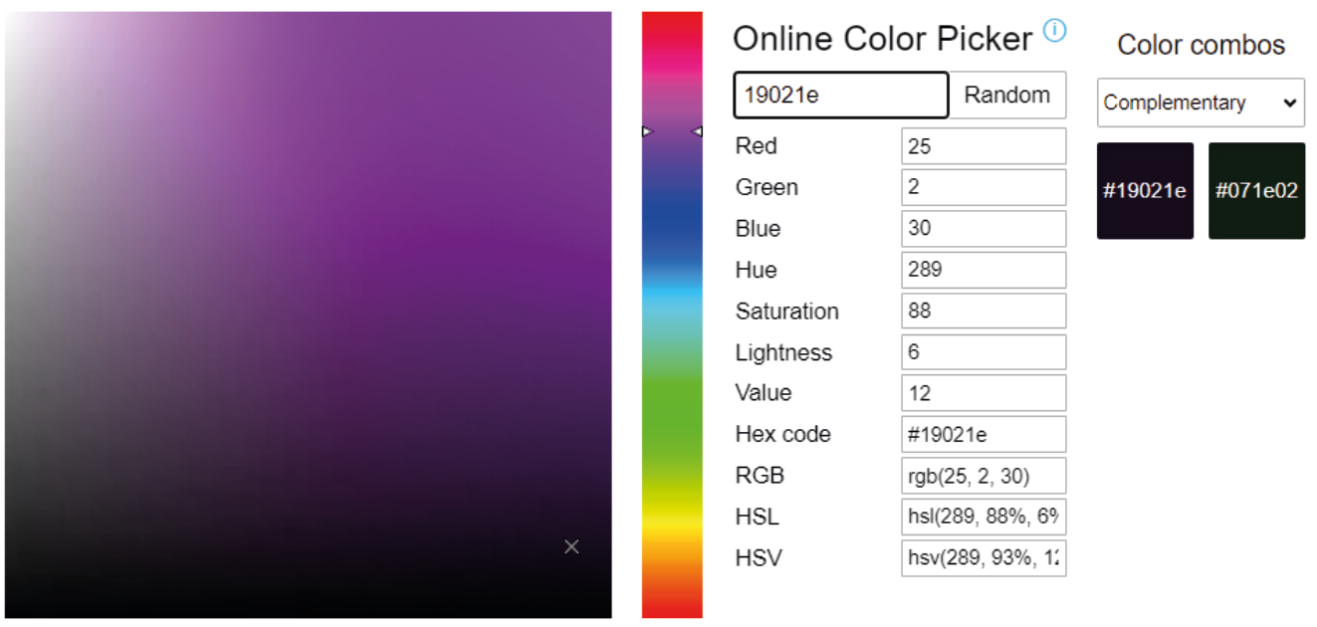
\includegraphics[width=0.8\textwidth]{IMG/color_picker.png}
    \caption{\texttt{colorpicker}}
    \label{fig:colorpicker}
\end{figure}

\subsection*{Indices}
\begin{itemize}
	\item[-] Le nombre hexadécimal d'une couleur représente ses valeurs \textit{RougeVertBleu} codées avec six nombres. Les deux premiers correspondent à la couleur rouge, les deux suivants au vert et les deux derniers au bleu. Pour transformer cette valeur hexadécimale en décimal, il vous suffit de convertir chacune des paires de ce nombre.
	\item[-] Vous pouvez vous aider de la librairie \texttt{colorsys} pour vous permettre de réaliser facilement les conversions.
	\item[-] Ce sont principalement les fonctions \texttt{colorsys.rgb\_to\_hls} et \texttt{colorsys.hls\_to \_rgb} qui pourront être utilisées. 
	\item[-] Pour chercher la complémentaire d’une couleur, il faut passer par le format \textit{TSL} en faisant une rotation de 180° sur la teinte et trouver ainsi la position de la couleur diamétralement opposée.
	\item[-] Pour faire une rotation, il faudra bien sûr penser à normaliser la valeur de la teinte \textit{TSL} qui par défaut est de \texttt{[0, 1]} en \texttt{[0°, 360°]} puis faire la rotation en additionnant avec 180°.
\end{itemize}
\medskip

\begin{figure}[h]
    \centering
    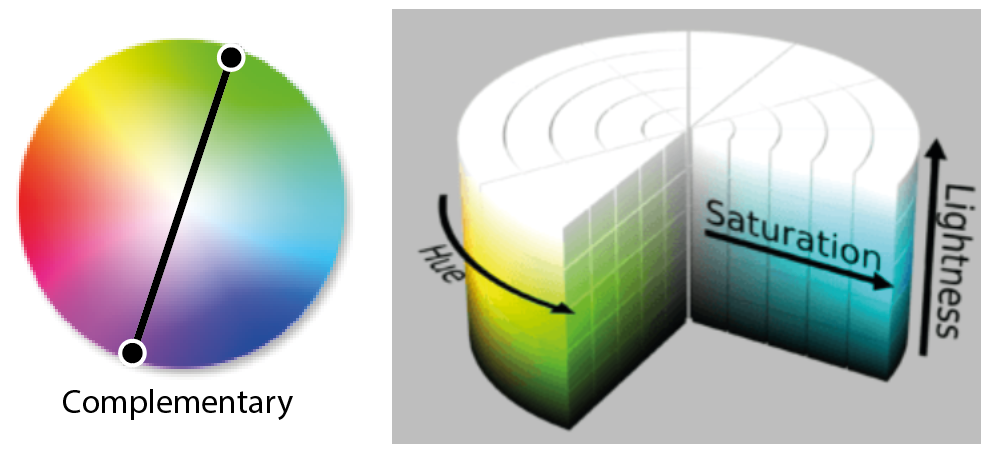
\includegraphics[width=0.8\textwidth]{IMG/schema_colors.png}
    \caption{Couleur complémetaire et TSL}
    \label{fig:colorpicker}
\end{figure}
\medskip

\section{Mon code}
\begin{lstlisting}
from colorsys import rgb_to_hls, hls_to_rgb


def get_color_types(color: str) -> dict:
    rvb = [int(color[i:i+2], 16) for i in
           range(1, len(color), 2)]
    tsl = list(rgb_to_hls(*list(map(lambda x: x/255,
                                    rvb))))
    tsl.insert(-1, tsl.pop())
    tsl_norm = (f"{round(tsl[0]*360)}°",
                *[f"{el:.0%}" for el in tsl[1:3]])
    return {"hex": color, "rvb": rvb,
            "tsl_norm": tsl_norm, "tsl": tuple(tsl)}


def get_complementary(color: str) -> str:
    t, s, l = get_color_types(color)["tsl"]
    return f'#{"".join([f"{round(el*255):02x}" for el 
                        in hls_to_rgb(t+.5 % 1, l, s)])}'
\end{lstlisting}
\medskip

\section{Explications}
\subsection*{Contexte}
Il s'agit soit de faire tous les calculs à la main pour les conversions entre les formats de couleur, soit trouver une bibliothèque qui nous permet de nous simplifier la vie. Mon choix s'est porté sur la bibliothèque \texttt{colorsys} qui est plutôt sympathique pour cela. Elle nous permet de passer au format \texttt{TSL} via \texttt{RGB} et vice et versa.
\medskip

Le but est aussi de trouver la couleur complémentaire, qui est la couleur diamétralement opposée sur le cercle chromatique. Pour cela \texttt{TSL}, nous permet de faire une rotation et trouver directement cette valeur sans difficulté particulière.
\medskip

\subsection*{Différentes problématiques}
\begin{description}
	\item[\textbullet{} Le dièze \og \texttt{\#}\fg{}... gênant hein !] : il y a donc plusieurs façon de faire, soit un simple \texttt{lstrip()} et hop viré, soit débuter son index à \texttt{1}.
	\item[\textbullet{} Conversion d'un format hexadécimal à un format décimal pour le \texttt{RVB}] : \\ un simple \texttt{int(..., 16)} nous fait le calcul directement !
	\item[\textbullet{} Normaliser ses valeurs] : avec la bibliothèque \texttt{colorsys}, attention à toujours rester dans un domaine de valeurs comprises entre \texttt{0} et \texttt{1}, comme stipulé dans la documentation officielle de \texttt{colorsys}\footnote{\url{https://docs.python.org/3/library/colorsys.html} : \og \texttt{the coordinates are all between 0 and 1...}\fg{}}.
	\item[\textbullet{} \texttt{HLS} vs \texttt{TSL}] : attention à bien penser à inverser la saturation de la luminosité si vous utilisez la bibliothèque \texttt{colorsys}.
	\item[\textbullet{} \textit{Tuple}, \textit{liste}] : l'énoncé précise de bien respecter les différents types dans le dictionnaire renvoyé par la fonction.
	\item[\textbullet{} Utilisation des fonctions déjà crées] : on a déjà développé la fonction \texttt{get\_color \\ \_type()} alors pourquoi ne pas l'utiliser pour créer la fonction \texttt{get\_complementar \\ y()} afin d'avoir directement la valeur \texttt{TSL}.
	\item[\textbullet{} Trouver la valeur diamétralement opposée] : une rotation de \texttt{180°} ou de \texttt{0.5} dans la plage de limites [\texttt{0} - \texttt{1}] puis un \textit{modulo} de \texttt{1} à appliquer pour rester dans cette plage de valeurs.
\end{description}
\medskip

\subsection*{Explication du code et astuces d'optimisation / \textit{refactoring}}
\begin{lstlisting}
rvb = [int(color[i:i+2], 16) for i in
           range(1, len(color), 2)]
\end{lstlisting}
\medskip

On pointe avec un \texttt{range} sur la chaîne de caractères \texttt{color} avec un index de \texttt{1} jusqu'à sa taille totale suivant un pas de \texttt{2}, puis avec \texttt{[i:i+2]} on vient chercher deux par deux les caractères hexadécimaux de chaque couleur à convertir en décimal.
\medskip

\begin{lstlisting}
tsl = list(rgb_to_hls(*list(map(lambda x: x/255, rvb))))
\end{lstlisting}
\medskip

Pour constituer notre \texttt{TSL}, on utilise la fonction \texttt{colorsys.rgb\_to\_hls()}. J'ai volontairement utilisé la fonction \texttt{map()} pour vous permettre de voir de nouvelles choses en plus de la compréhension de liste. Ceci \texttt{list(map(lambda x: x/255, rvb))} est la même chose que cela : \texttt{[x/255 for x in rvb]}. C'est juste une autre façon de faire ! Donc on vient diviser chaque couleur \texttt{R}, \texttt{V} et \texttt{B} par \texttt{255} pour respecter la norme \texttt{0} à \texttt{1} qui sera nécessaire pour l'argument de la fonction \texttt{rgb\_to\_hls()}. Notez l'astérisque (\texttt{*}) qui permet de faire un \textit{unpacking} pour dispatcher les éléments \texttt{RVB} en trois arguments, la fonction \texttt{rgb\_to\_hls()} nécessitant trois arguments pour fonctionner. Et l'on convertit en \texttt{list()} car nous avons ensuite besoin d'intervertir les deux derniers éléments, luminosité et saturation étant inversés par rapport à l'énoncé du challenge.
\medskip

\begin{lstlisting}
tsl.insert(-1, tsl.pop())
\end{lstlisting}
\medskip

C'est la phrase magique qui permet d'inverser les places des deux derniers éléments de la liste. \texttt{pop()} permet de retirer le dernier élément, 
\texttt{insert()} permet d'insérer ce que \texttt{pop()} renvoie à l'index \texttt{-1}, qui est l'avant dernière position... \texttt{-1} étant la dernière position mais l'insertion se passe juste avant la position indiquée, donc juste avant \texttt{-1}. La liste \texttt{tsl} sera alors modifiée directement.
\medskip

\begin{lstlisting}
tsl_norm = (f"{round(tsl[0]*360)}°",
                *[f"{el:.0%}" for el in tsl[1:3]])
\end{lstlisting}
\medskip

On utilise le résultat de la conversion \texttt{TSL} pour obtenir \texttt{TSL\_norm}:
\begin{itemize}
	\item[-] La teinte est définie en degrés, comprise dans une limite entre 0 et 360°. \texttt{round()} permet d'arrondir pour avoir une valeur sans chiffre après la virgule. 
	\item[-] La luminosité et la saturation quant à elles sont exprimées en pourcentage grâce à l'utilisation d'une \textit{f-string} qui avec \og \texttt{\%}\fg{} permet à la fois de multiplier par \texttt{100} et d'afficher le pourcentage. Le \texttt{.0} permet de supprimer les chiffres après la virgule. \texttt{tsl[1:3]} c'est la lecture des élément \texttt{1} et \texttt{2} de la liste \texttt{tsl}. On utilise encore l'astérisque (\texttt{*}) pour avoir en tout trois arguments pour \texttt{tsl\_norm}.
\end{itemize}
\medskip

\begin{lstlisting}
return {"hex": color, "rvb": rvb,
            "tsl_norm": tsl_norm, "tsl": tuple(tsl)}
\end{lstlisting}
\medskip

Juste un simple \texttt{return} pour renvoyer un dictionnaire. Notez le \texttt{tuple()} qui permet de convertir notre précédente liste en tuple afin de suivre l'énoncé du challenge.
\medskip

\begin{lstlisting}
t, s, l = get_color_types(color)["tsl"]
\end{lstlisting}
\medskip

On envoie le résultat \textit{TSL} du dictionnaire de la fonction précédente dans les variables \texttt{t}, \texttt{s} et \texttt{l}. Il est important d'utiliser \texttt{tsl} plutôt que \texttt{tsl\_norm} afin de travailler sur des valeurs non arrondies et avoir ainsi plus de précision.
\medskip

\begin{lstlisting}
return f'#{"".join([f"{round(el*255):02x}" for el 
                        in hls_to_rgb(t+.5 % 1, l, s)])}'
\end{lstlisting}
\medskip

Ce \texttt{return} peut paraître un peu complexe mais tout deviendra simple une fois décomposé :
\medskip

\begin{verbatim}
t+.5 % 1
\end{verbatim}
\medskip

On effectue une rotation de la teinte de \texttt{180°} mais comme on se trouve dans un espace compris entre 0 à 1, alors cela devient \texttt{180/360 = 1/2 = 0.5}. Pour rester dans la norme, on fait un \textit{modulo} \texttt{1}.
\medskip

\begin{verbatim}
hls_to_rgb(t+.5 % 1, l, s)
\end{verbatim}
\medskip

On convertit en \textit{RVB} via \textit{TSL}, avec la teinte, la luminosité et la saturation.
\medskip

\begin{verbatim}
[f"{round(el*255):02x}" for el in hls_to_rgb(t+.5 % 1, l, s)]
\end{verbatim}
\medskip

Cette compréhension de liste nous fournit le \textit{RVB} au format hexadécimal. Il faut pour ça changer la norme et passer de \texttt{[0-1]} à \texttt{[0-255]} en multipliant par \texttt{255} puis convertir en hexadécimal via \texttt{02x}, ce qui nous donne deux chiffres (les valeurs de 0 à 9 seront écrites à l'aide de deux chiffres : 01 02 03 04... 09), \texttt{x} permet la conversion grâce à une \textit{f-string}.
\medskip

\begin{verbatim}
f'#{"".join([f"{round(el*255):02x}" for el 
                        in hls_to_rgb(t+.5 % 1, l, s)])}'
\end{verbatim}
\medskip

\texttt{"".join()} permet de réunir le résultat de chaque paire \textit{RVB}/\textit{hexadécimal} et enfin le \og \texttt{\#}\fg{}, la cerise sur le gâteau !
\medskip

\subsection*{Mon fichier d'\textit{unitests}}
\begin{lstlisting}
import pytest

@pytest.mark.parametrize("hexcode, expected", [
    ("#19021e", {'hex': '#19021e', 'rvb': [25, 2, 30],
                 'tsl_norm': ('289°', '88%', '6%'),
                 'tsl': (0.8035714285714285, 0.875,
                         0.06274509803921569)}),
    ("#aedd5f", {'hex': '#aedd5f', 'rvb': [174, 221, 95],
                 'tsl_norm': ('82°', '65%', '62%'),
                 'tsl': (0.22883597883597884,
                         0.6494845360824743,
                         0.6196078431372549)}),
    ("#ff0000", {'hex': '#ff0000', 'rvb': [255, 0, 0],
                 'tsl_norm': ('0°', '100%', '50%'),
                 'tsl': (0.0, 1.0, 0.5)})
])
def test_different_colour_writing_formats(
        hexcode, expected):
    got = get_color_types(hexcode)

    assert got == expected

@pytest.mark.parametrize("hexcode, expected", [
    ("#19021e", "#071e02"),
    ("#aedd5f", "#8e5fdd"),
    ("#ff0000", "#00ffff"),
])
def test_for_complementary_color_in_hex(
        hexcode, expected):
    got = get_complementary(hexcode)
\end{lstlisting}
\medskip

\subsection*{Quelques conseils}
\begin{itemize}
	\item[\textbullet] Faire fonctionner son code le plus tôt possible en évitant les problèmes.
	\item[\textbullet] Coder simplement pour obtenir un premier jet et optimiser/refactoriser par la suite
	\item[\textbullet] Ne pas hésiter pas à s'aider de bibliothèques, mais il est possible de réaliser tous les calculs à la main pour s'entraîner si on le souhaite.
	\item[\textbullet] Le but n'est pas d'obtenir le code le plus court, mais un code lisible et optimisé avec un algorithme efficace. Penser qu'un code n'est pas seulement pour son usage personnel, surtout si on travaille en \textit{open source}, donc veiller a ce qu'il soit clair. Ne pas hésiter à ajouter des commentaires, cela nous servira tout autant quand nous reverrons notre code trois mois plus tard sans y avoir touché !
\end{itemize}
\medskip

\chapter{Calculatrice romaine}
\vspace{2cm}
\section{Énoncé}
Le but de ce challenge est de développer la fonction:
\begin{verbatim}
add_romans(calculate:str)->str
\end{verbatim}
...qui permet de calculer la somme de deux ou plusieurs nombres écrits en chiffres romains\footnote{\url{https://fr.wikipedia.org/wiki/Num\%C3\%A9ration_romaine)}}.

\subsection*{Conditions}
\begin{itemize}
	\item[-] L'affichage du prompt se fera via la console.
	\item[-] L'opération est simple : deux ou plusieurs nombres écrits sur une seule ligne en chiffres romains séparés par un signe \texttt{+}.
	\item[-] Le résultat de l'opération sera bien sûr donné en chiffres romains dans une plage comprise entre \texttt{I} et \texttt{MMMCMXCIX}.
	\item[-] Vérifier que les chiffres romains et l'opération entrés par l'utilisateur sont valides. Les lettres doivent toujours êtres écrites en majuscules.
	\item[-] Les chiffres romains sont : \texttt{IVXLCDM}.
	\item[-] \texttt{I}, \texttt{X} et \texttt{C} ne peuvent pas être répétés plus de trois fois.
	\item[-] \texttt{V}, \texttt{L} et \texttt{D} ne peuvent pas apparaître plus d'une fois.
\end{itemize}
\medskip

\subsection*{Exemples}
\begin{verbatim}
- X + IV -> XIV
- MXCIX + CIV -> MCCIII
- II + II -> IV
- MMMCX + DCII -> MMMDCCXII
- MCMXCIX + I -> MM
- IVM + I -> erreur (IVM n'est pas valide)
- VVI -> erreur (2x V n'est pas valide)
- XXXX -> erreur (4x X n'est pas valide)
- TX -> erreur (T ne fait pas partie de la liste des chiffres romains)
- XX - IV -> erreur (seule l'addition est permise)
- IV -> erreur (2 éléments minimum) 
- MMMCMXC + X -> erreur (débordement, doit respecter la plage de I à 
MMMCMXCIX inclus)
\end{verbatim}
\medskip

\subsection*{Ressource}
Voir le site \texttt{Roman numerals calculator} pour réaliser des tests\footnote{\url{https://www.hackmath.net/en/calculator/roman-numerals}}.
\medskip

\section{Ma proposition}
\begin{lstlisting}
from re import search

ROMANS = {"I": 1, "V": 5, "X": 10, "L": 50,
          "C": 100, "D": 500, "M": 1000}
SPEC = {4: ("IV", "XL", "CD"), 9: ("IX", "XC", "CM")}
list_romans = list(ROMANS.keys())


def to_dec(roman_nb: str) -> int:
    nb = [ROMANS[el] for el in roman_nb]
    return sum([nb[i] - 2 * nb[i - 1] if nb[i] > nb[i - 1]
                else nb[i] for i in
                range(1, len(nb))]) + nb[0]


def n_to_9(nb: int, lv: int) -> str:
    base, v = list_romans[lv * 2], list_romans[1:6:2][lv]
    return f"{base * nb}" if nb < 4 else v if nb == 5 \
        else SPEC[nb][lv] if nb in SPEC \
        else f"{v}{base * (nb - 5)}"


def to_roman(nb: int) -> str:
    nb = [int(i) for i in reversed(str(nb))]
    return "".join([f"{'M' * nb[3]}" if i == 3
                    else n_to_9(nb[i], i) for i in
                    range(0, len(nb))][::-1])


def add_romans(calculate: str) -> str:
    if [el for el in "-*/" if el in calculate]:
        return "Seule l'addition est permise"

    el_list = calculate.replace(" ", "").split("+")
    if len(el_list) < 2:
        return "2 éléments minimum"

    calc = []
    for el in el_list:
        err = [lt for lt in el if lt not in ROMANS]
        if err:
            return (f"{err[0][0]} ne fait pas partie de "
                    f"la liste des chiffres romains")

        if search("IL|IC|ID|IM|XD|XM|VL|VC|VD|VM", el):
            return f"{el} n'est pas valide"

        err = search("V.*?V|L.*?L|D.*?D", el)
        if err:
            return f"2x {err[0][0]} n'est pas valide"

        err = search(
            rf'([{"".join(list_romans[0:5:2])}])\1{{3,}}',
            el)
        if err:
            return f"4x {err[0][0]} n'est pas valide"

        err = search(
            rf'({"|".join(SPEC[4] + SPEC[9])}).*?\1', el)
        if err:
            return f"2x {err[0]} n'est pas valide"

        calc.append(to_dec(el))
    result = sum(calc)
    return to_roman(result) if result < 4000 else \
        ("Débordement, doit respecter la plage de I à "
         "MMMCMXCIX inclus")


if __name__ == '__main__':
    print(add_romans(input("une opération : ")))
\end{lstlisting}
\medskip

\subsection*{Mon fichier d'\textit{unitests}}
\begin{lstlisting}
import pytest

@pytest.mark.parametrize("calculate, expected", [
    ("X + IV", "XIV"),
    ("MXCIX + CIV", "MCCIII"),
    ("II + II", "IV"),
    ("MMMCX + DCII", "MMMDCCXII"),
    ("MCMXCIX + I", "MM"),
    ("IVM + I", "IVM n'est pas valide"),
    ("VVI + I", "2x V n'est pas valide"),
    ("XXXX + I", "4x X n'est pas valide"),
    ("TX + I", "T ne fait pas partie de la liste des "
               "chiffres romains"),
    ("XX - IV", "Seule l'addition est permise"),
    ("IV", "2 éléments minimum"),
    ("MMMCMXC + X", "Débordement, doit respecter la plage "
                    "de I à MMMCMXCIX inclus"),
])
def test_should_return_the_sum_of_roman_numbers(calculate,
                                                expected):
    got = add_romans(calculate)

    assert got == expected

\end{lstlisting}
\medskip

\section{Explications}
\subsection*{Contexte}
Il s'agit de trouver un moyen pour additionner des chiffres romains entre eux.  Pour cela, il est préférable de rester dans un domaine de nombres arabes pour effectuer l'opération arithmétique puis reconvertir la sommes finales en chiffres romains.
\medskip

\subsection*{Les différentes problématiques}
\begin{itemize}
	\item[\textbullet] \textbf{Conversion chiffres romains en chiffres arabes :} Il faut trouver une astuce pour faire correspondre ces chiffres romains en chiffres arabes. La solution est dans cette phrase : \og \textit{Un nombre écrit en chiffres romains se lit de gauche à droite. En première approximation, sa valeur se détermine en faisant la somme des valeurs individuelles de chaque symbole, sauf quand l'un des symboles précède un symbole de valeur supérieure ; dans ce cas, on soustrait la valeur du premier symbole au deuxième}\fg{}\footnote{Source \texttt{Wikipédia}: \url{https://fr.wikipedia.org/wiki/Numération_romaine}}.
	\item[\textbullet] \textbf{Conversion du résultat en chiffres romains :} Il y a plusieurs façons de faire, soit faire correspondre chaque symbole romain, soit reconstituer le nombre par dizaine, centaine et millier.
	\item[\textbullet] \textbf{Gestion des erreurs :} Pour ce challenge, il s'agissait de simplement suivre la liste dans les exemples, car plusieurs écritures sont possible en fonction de la version romaine utilisée. Dans ce cas, faire un simple \texttt{return} du texte est accepté, sinon faire l'habituel \texttt{raise} pour \textit{lever l'erreur}.
\end{itemize}
\medskip

\subsection*{Explication du code}
Mon programme se divise donc en trois, voire en quatre parties :
\medskip

\subsubsection*{La conversion des chiffres romains en chiffres arabes}
Avec la fonction :
\begin{verbatim}
to_dec(roman_nb:str)->int
\end{verbatim}
\medskip

Ici, de simples additions tant qu'on ne rencontre pas de paires contenant un élément de valeur supérieur, auquel cas, il faudra réaliser une soustraction.
La conversion s'opère principalement par ces lignes :
\begin{lstlisting}
def to_dec(roman_nb: str) -> int:
    nb = [ROMANS[el] for el in roman_nb]
    return sum([nb[i] - 2 * nb[i - 1] if nb[i] > nb[i - 1]
                else nb[i] for i in
                range(1, len(nb))]) + nb[0]
\end{lstlisting}
\medskip

\subsubsection*{La conversion des chiffres arabes en chiffres romains} 
Avec la fonction :
\begin{verbatim}
to_roman(nb:int)->str
\end{verbatim}
\medskip

Là, c'est plus compliqué. Ici je décompose mon nombre en unité, dizaine, centaine et millier et m'occupe de chaque éléments un par un. Les éléments particulier 4, 5 et 9 sont traités dans une sous-fonction :
\begin{lstlisting}
def n_to_9(nb: int, lv: int) -> str:
    base, v = list_romans[lv * 2], list_romans[1:6:2][lv]
    return f"{base * nb}" if nb < 4 else v if nb == 5 \
        else SPEC[nb][lv] if nb in SPEC \
        else f"{v}{base * (nb - 5)}"
\end{lstlisting}
\medskip

Le code de la fonction est le suivant :
\begin{lstlisting}
def to_roman(nb: int) -> str:
    nb = [int(i) for i in reversed(str(nb))]
    return "".join([f"{'M' * nb[3]}" if i == 3
                    else n_to_9(nb[i], i) for i in
                    range(0, len(nb))][::-1])
\end{lstlisting}
\medskip

\subsubsection*{La fonction principale}
\begin{verbatim}
add_romans(calculate:str)->str
\end{verbatim}
\medskip

Corps du programme dans lequel la gestion des erreurs se fait à l'aide principalement des \textit{expressions régulières} (\textit{regex}).
\begin{lstlisting}
def add_romans(calculate: str) -> str:
    if [el for el in "-*/" if el in calculate]:
        return "Seule l'addition est permise"

    el_list = calculate.replace(" ", "").split("+")
    if len(el_list) < 2:
        return "2 éléments minimum"

    calc = []
    for el in el_list:
        err = [lt for lt in el if lt not in ROMANS]
        if err:
            return (f"{err[0][0]} ne fait pas partie de "
                    f"la liste des chiffres romains")

        if search("IL|IC|ID|IM|XD|XM|VL|VC|VD|VM", el):
            return f"{el} n'est pas valide"

        err = search("V.*?V|L.*?L|D.*?D", el)
        if err:
            return f"2x {err[0][0]} n'est pas valide"

        err = search(
            rf'([{"".join(list_romans[0:5:2])}])\1{{3,}}',
            el)
        if err:
            return f"4x {err[0][0]} n'est pas valide"

        err = search(
            rf'({"|".join(SPEC[4] + SPEC[9])}).*?\1', el)
        if err:
            return f"2x {err[0]} n'est pas valide"

        calc.append(to_dec(el))
    result = sum(calc)
    return to_roman(result) if result < 4000 else \
        ("Débordement, doit respecter la plage de I à "
         "MMMCMXCIX inclus")
\end{lstlisting}
\medskip

\subsubsection*{Notes sur les \textit{regexes} utilisées}
Le \textit{regex} est un langage à part entière, il permet de chercher des occurrences plus ou moins complexes dans un bloc de texte. C'est grâce à la bibliothèque \texttt{re} que l'on peut l'intégrer facilement à \textit{Python}.
\begin{verbatim}
search("IL|IC|ID|IM|XD|XM|VL|VC|VD|VM", el)
\end{verbatim}

\texttt{search} cherche soit \texttt{IL}, \texttt{IC}, \texttt{ID}, \texttt{IM}... le caractère \og \texttt{$|$}\fg{} représente le \og \texttt{or}\fg{}.
\medskip

\begin{verbatim}
search("V.*?V|L.*?L|D.*?D", el)
\end{verbatim}
\medskip

Cela représente n'importe quel caractère (\texttt{*?} signifie \og \textit{jusqu'à}\fg{}. Donc de \texttt{V} jusqu'à \texttt{V}, ce qui permet d'indiquer que deux \texttt{V} peuvent être présents. De même à l'aide de \og or\fg{} pour chercher aussi deux \texttt{L} et deux \texttt{D}.
\medskip

\begin{verbatim}
search(rf'([{"".join(list_romans[0:5:2])}])\1{{3,}}', el)
\end{verbatim} ‎
\medskip

\texttt{list\_romans[0:5:2]} correspond à \texttt{["I", "X", "C"]}. On réalise  ici un \texttt{.join()}, ce qui nous donne \texttt{IXC}. Ce \texttt{IXC} est entre parenthèses car nous faisons ainsi un groupe qui enregistre le caractère trouvé entre \texttt{I} ou \texttt{X} ou \texttt{C}. Le \texttt{\textbackslash{}1} permet de récupérer ce groupe et recherche alors les deux mêmes caractères qui se suivent. \texttt{\{3,\}} veut dire : répéter au moins trois ou plus. Donc en tout, on cherche la répétition du même caractère quatre fois de suite (une fois dans le premier groupe, puis trois fois à l'aide de \texttt{\textbackslash{}1}).
\medskip

\begin{verbatim}
search(rf'({"|".join(SPEC[4]+SPEC[9])}).*?\1', el)
\end{verbatim}
\medskip

On cherche si \texttt{SPEC[4]} est dans \texttt{("IV", "XL", "CD")} ou si \texttt{SPEC[9]} est dans ("IX", "XC", "CM"), et s'ils sont présents deux fois. Pour information, le \texttt{r} avant le \texttt{f} du \textit{f-string} permet d'ignorer le caractère d'échappement \og \texttt{\textbackslash{}}\fg{}, car sans ce \texttt{r} il aurait fallu écrire \og \texttt{\textbackslash{}\textbackslash{}1}\fg{} plutôt que \og \texttt{\textbackslash{}1}\fg{}.
\medskip

\section{En complément}
\begin{itemize}
	\item[-] A noter deux vidéos existantes sur le sujet présentes sur \texttt{Youtube}: \textit{Convertir des nombres entiers en chiffres romains}\footnote{\url{https://www.youtube.com/watch?v=fD9aw0dZtjc}} et \textit{Convertir des chiffres romains en nombres entiers}\footnote{\url{https://www.youtube.com/watch?v=WFyrryNO9Nk}}.
	\item[-] \textit{Comment vérifier si une liste est vide en Python ?}\footnote{\url{https://flexiple.com/python/check-if-list-is-empty-python}}
\end{itemize}
\medskip


\chapter{Affichage digital 7 segments}
\vspace{2cm}
\section{Énoncé}
Le but de ce challenge est de développer la fonction \texttt{digital\_time()->str} qui retourne l'heure actuelle au format d'affichage digital à sept segments\footnote{\url{https://fr.wikipedia.org/wiki/Affichage_\%C3\%A0_sept_segments}}.
\medskip

\subsection*{Étapes}
\begin{enumerate}
	\item Transcrire les chiffres de 0 à 9 en sept segments digitaux.
	\item Transcrire plusieurs chiffres à la suite sur une seule ligne.
	\item Afficher l'heure en la retranscrivant.
\end{enumerate}
\medskip

\subsection*{Conditions}
\begin{itemize}
	\item[-] L'affichage se fait via la console
	\item[-] L'heure doit être affichée au format 24h.
	\item[-] L'heure et les minutes sont séparées par deux points, le tout sur une même ligne d'affichage avec deux espaces de séparation.
	\item[-] Le résultat de l'affichage de l'heure actuelle doit correspondre aux exemples ci-dessous à l'aide du caractère \og \texttt{\#}\fg{}.
	\item[-] Les sept segments \texttt{a}, \texttt{b}, \texttt{c}, \texttt{d}, \texttt{e}, \texttt{f}, \texttt{g} sont les suivants :
	\newpage
	
	\begin{verbatim}
     a
     v 
    ####   
f-> #  # <- b
    #### <- g
e-> #  # <- c
    ####
     ^
     d
	\end{verbatim}
	\item[-] Pour des raisons d'ergonomie et d'esthétisme, les segments se superposent et s'affichent de manière plus allongée, ainsi le chiffre \texttt{2} s'affichera de la façon suivante:
	\begin{verbatim}
	
             ####                        ##
                #                          #
comme ceci : ####   et pas comme cela :  ## 
             #                          #
             ####                        ##	
	\end{verbatim}
\end{itemize}
\medskip

\subsection*{Exemples}
\begin{itemize}
	\item[-] À \texttt{17h26}, le résultat de \texttt{digital\_time()} donne :
	\begin{verbatim}
	#  ####     ####  ####
	#     #  #     #  #  
	#     #     ####  ####
	#     #  #  #     #  #
	#     #     ####  ####
	\end{verbatim}
	\medskip
	
	\item[-] À \texttt{23h59}, le résultat de \texttt{digital\_time()} donne :
	\begin{verbatim}
	####  ####     ####  ####
	   #     #  #  #     #  #
	####  ####     ####  ####
	#        #  #     #     #
	####  ####     ####  ####
	\end{verbatim}
	\medskip
	
	\item[-] À \texttt{4h08}, le résultat de \texttt{digital\_time()} donne :
-	\begin{verbatim}
	#  #     ####  ####
	#  #  #  #  #  #  #
	####     #  #  ####
	   #  #  #  #  #  #
	   #     ####  ####
	\end{verbatim}
\end{itemize}
\medskip

\section{Ma proposition avec l'utilisation de \texttt{Numpy}}
\begin{lstlisting}
from numpy import hstack, delete, full, ndarray
from datetime import datetime

SEG_MAP = (((0, 0), (0, 1), (0, 2), (0, 3)),  # a
           ((0, 3), (1, 3), (2, 3)),  # b
           ((2, 3), (3, 3), (4, 3)),  # c
           ((4, 0), (4, 1), (4, 2), (4, 3)),  # d
           ((4, 0), (3, 0), (2, 0)),  # e
           ((2, 0), (1, 0), (0, 0)),  # f
           ((2, 0), (2, 1), (2, 2), (2, 3)),  # g
           ((1, 0), (3, 0)))


def display(el: str) -> ndarray:
    digit = full((5, 6), [" "], dtype=str)
    match el:
        case " ": return digit
        case ":":
            s = [*[0]*7, 1]
            digit = delete(digit, slice(3), 1)
        case _:
            b = [int(b) for b in f"{int(el):04b}"][::-1]
            s = (b[3] or b[1] or b[0] and b[2] or not b[0]
                 and not b[2],
                 b[0] and b[1] or not b[1] and not b[0]
                 or not b[2],
                 b[2] or b[3] or not b[1] or b[0],
                 b[3] or b[1] and not b[0] or not b[2]
                 and not b[0] or not b[1] and b[0] and b[2]
                 or b[1] and not b[2],
                 b[1] and not b[0] or not b[0]
                 and not b[2],
                 b[3] or not b[0] and b[2] or not b[1]
                 and b[2] or not b[1] and not b[0],
                 b[3] or b[1] and not b[0] or not b[1]
                 and b[2] or not b[2] and b[1])
    digit[*zip(*[(r, c) for i, el in enumerate(s) if el
                 for r, c in SEG_MAP[i]])] = "#"
    return digit


def digital_time():
    time = datetime.now().strftime("%H:%M").lstrip("0")
    return "\n".join("".join(r) for r in
                     hstack([display(el) for el in
                             (time if len(time) == 5 else 
                              " " + time)]))


if __name__ == "__main__":
    print(digital_time())
\end{lstlisting}
\medskip

\section{Explications}
\subsection*{Contexte}
Il s'agit de trouver le moyen d'afficher un nombre sous forme digitale en sept segments comme on peut le voir sur certaines horloges numériques, puis d'afficher l'heure actuelle.
\medskip

\subsection*{Différentes problématiques}
\begin{itemize}
	\item[\textbullet] \textbf{Conversion d'un chiffre en sept segments pour simuler un affichage digital}: Il s'agit de repérer la position de chacun des segments puis \og d'allumer\fg{} les segments spécifiques au chiffre à afficher.
	\medskip
	
	\item[\textbullet] \textbf{Afficher plusieurs chiffres sur une ligne}: L'étape suivante est d'afficher plusieurs chiffres sur une même ligne en transposant les \og matrices\fg{} des chiffres à afficher.
	\medskip
	
	\item[\textbullet] \textbf{Ajouter le séparateur heure/minute}: Il nous faut donc ajouter le caractère \og \texttt{:}\fg{} entre les heures et les minutes.
	\medskip
	
	\item[\textbullet] \textbf{Formatage particulier}: Les heures de 0 à 9 ne doivent pas afficher un zéro mais laisser l'espace d'un \textit{digit} à gauche.
\end{itemize}
\medskip

\subsection*{Explication du code}
Le code se divise en trois, voire quatre parties :
\medskip

\subsubsection*{\textbullet{} Définir les segments à allumer en fonction du chiffre à afficher}
Ma méthode ici consiste à chercher des solutions combinatoires pour chaque segment en fonction du chiffre à afficher. Les chiffres sont au nombre de 10 et peuvent varier de 0 à 9. Ce qui nécessite quatre \textit{bits} pour les coder en binaire :
\begin{verbatim}
0000 -> 0
0001 -> 1
0010 -> 2
...
1000 -> 8
1001 -> 9
\end{verbatim}
\medskip

Il y a ensuite sept solutions combinatoires à rechercher pour chacun des segments de \og \texttt{a}\fg{} à \og \texttt{g}\fg{}.
\begin{figure}[h]
    \centering
    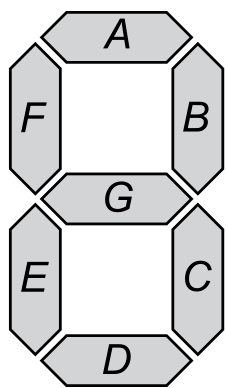
\includegraphics[width=0.2\textwidth]{IMG/sept_segments.png}
    \caption{Représentation visuelle des sept solutions combinatoires}
    \label{fig:colorpicker}
\end{figure}
\medskip

Ainsi il faut allumer les segments \texttt{B} et \texttt{C} pour coder le chiffre \texttt{1}, \texttt{BCFG} pour le chiffre \texttt{4}, \texttt{ABCDEF} pour le chiffre \texttt{0}, etc. On peut donc poser tous ces résultat dans une \textit{table de vérité} :
\begin{figure}[h]
    \centering
    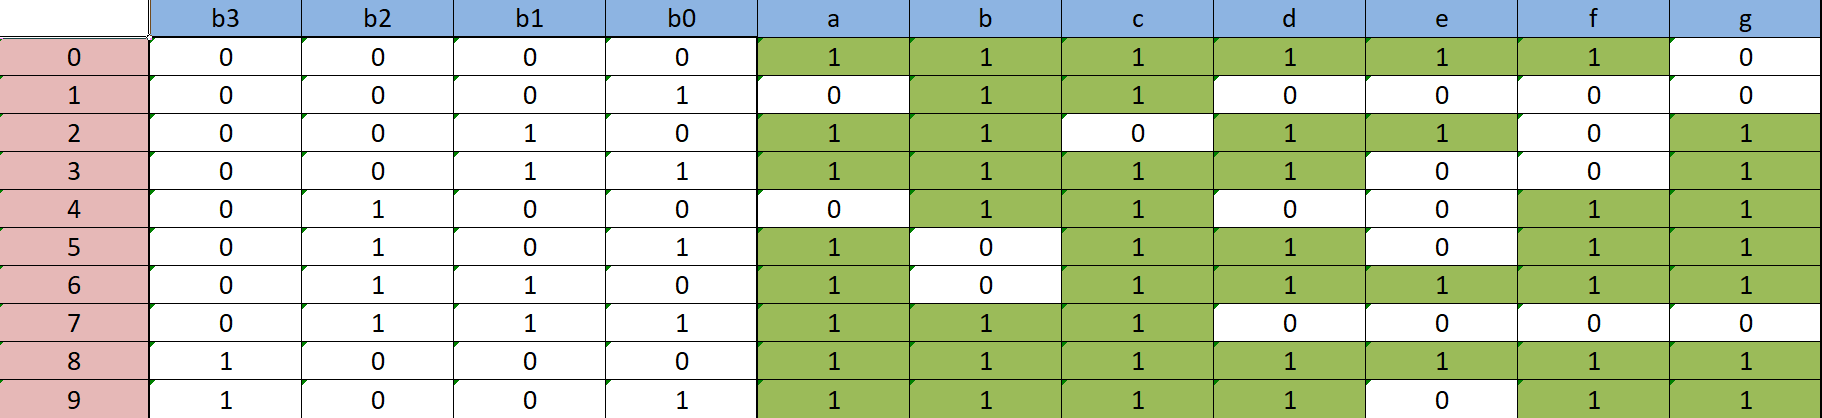
\includegraphics[width=0.9\textwidth]{IMG/table_de_verite.png}
    \caption{\textit{Table de vérité}}
    \label{fig:colorpicker}
\end{figure}
\medskip

A gauche les chiffres transcrits en quatre \textit{bits} de \texttt{b0} à \texttt{b3} et à droite les segments à allumer.
\medskip

La table de vérité est incomplète dans le sens où on n'utilise pas la totalité des possibilités en quatre \textit{bits}. Ainsi, on pourra être libre de choisir n'importe quels états durant la simplification de nos équations à l'aide des \textit{tableaux de Karnaugh} (ces combinaisons seront notées en rouge dans les tableaux).
\medskip

Le chiffre est d'abord converti en binaire sur quatre \textit{bits} pour procéder au calcul avec l'\textit{algèbre de Boole }:
\begin{verbatim}
b = [int(b) for b in f"{int(el):04b}"][::-1]
\end{verbatim}
\medskip

Pour faire bien correspondre à mes tableaux je suis obliger de faire une inversion via \texttt{[::-1]}.
\newpage

Pour simplifier chacune des sept solutions on posera nos \textit{tableaux de Karnaugh}\footnote{\textit{Tableaux de Karnaugh} - simplification d'expression en \textit{algèbre de Boole}: \url{https://www.youtube.com/watch?v=2tULBk6V9ZE}} de cette manière :
\begin{figure}[h!]
    \centering
    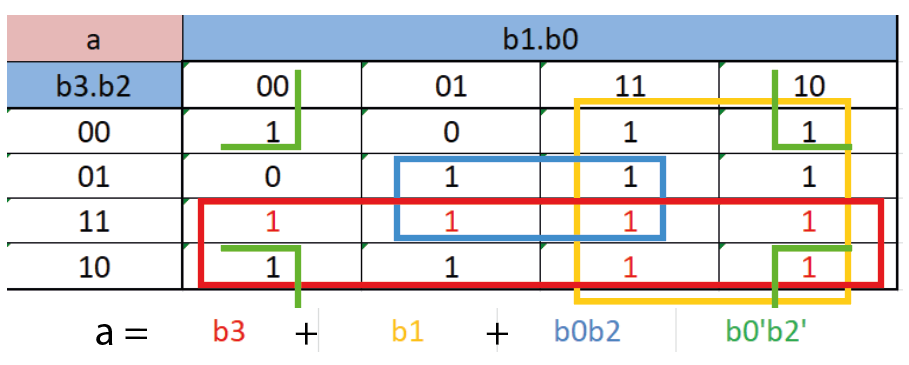
\includegraphics[width=0.9\textwidth]{IMG/tab_de_K_1.png}
    \caption{\textit{Tableau de Karnaugh} - 1}
    \label{fig:colorpicker}
\end{figure}
\medskip

\begin{figure}[h!]
    \centering
    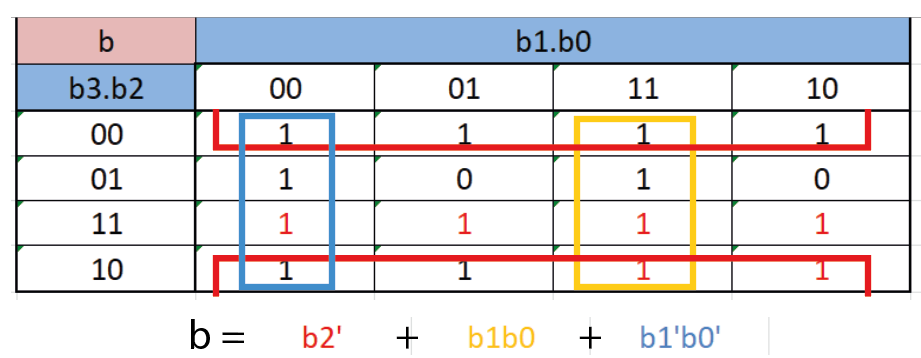
\includegraphics[width=0.9\textwidth]{IMG/tab_de_K_2.png}
    \caption{\textit{Tableau de Karnaugh} - 2}
    \label{fig:colorpicker}
\end{figure}
\medskip

\begin{figure}[h!]
    \centering
    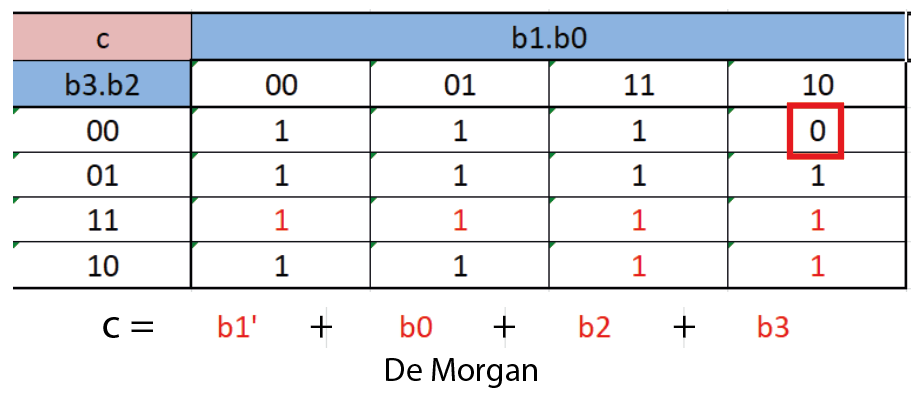
\includegraphics[width=0.9\textwidth]{IMG/tab_de_K_3.png}
    \caption{\textit{Tableau de Karnaugh} - 3}
    \label{fig:colorpicker}
\end{figure}
\newpage

\begin{figure}[h!]
    \centering
    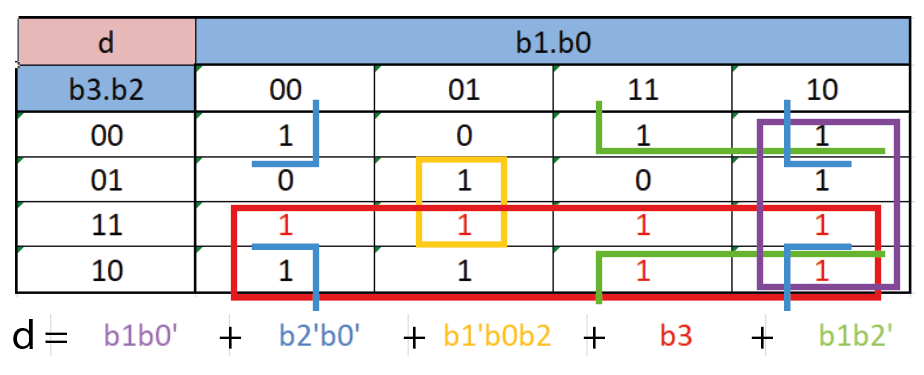
\includegraphics[width=0.9\textwidth]{IMG/tab_de_K_4.png}
    \caption{\textit{Tableau de Karnaugh} - 4}
    \label{fig:colorpicker}
\end{figure}
\medskip

\begin{figure}[h!]
    \centering
    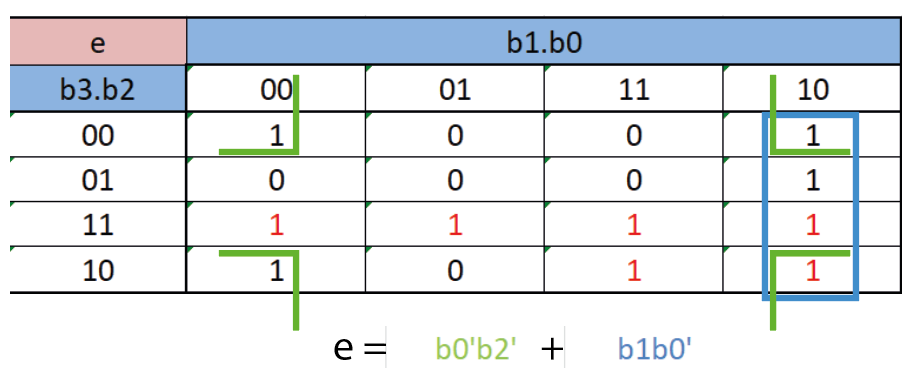
\includegraphics[width=0.9\textwidth]{IMG/tab_de_K_5.png}
    \caption{\textit{Tableau de Karnaugh} - 5}
    \label{fig:colorpicker}
\end{figure}
\medskip

\begin{figure}[h!]
    \centering
    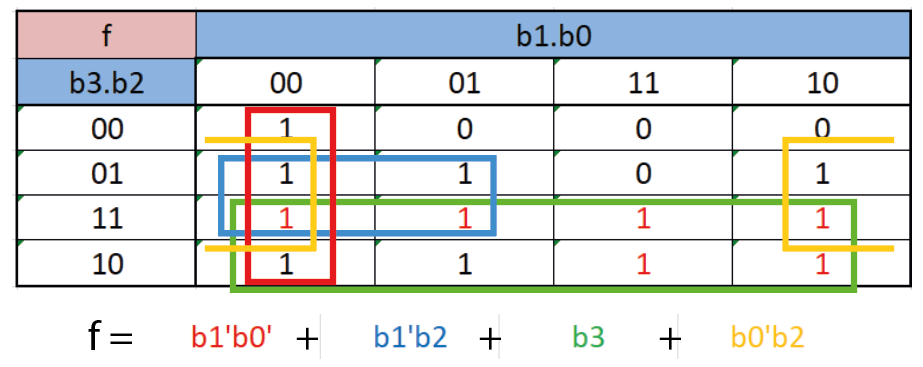
\includegraphics[width=0.9\textwidth]{IMG/tab_de_K_6.png}
    \caption{\textit{Tableau de Karnaugh} - 6}
    \label{fig:colorpicker}
\end{figure}
\newpage

\begin{figure}[h!]
    \centering
    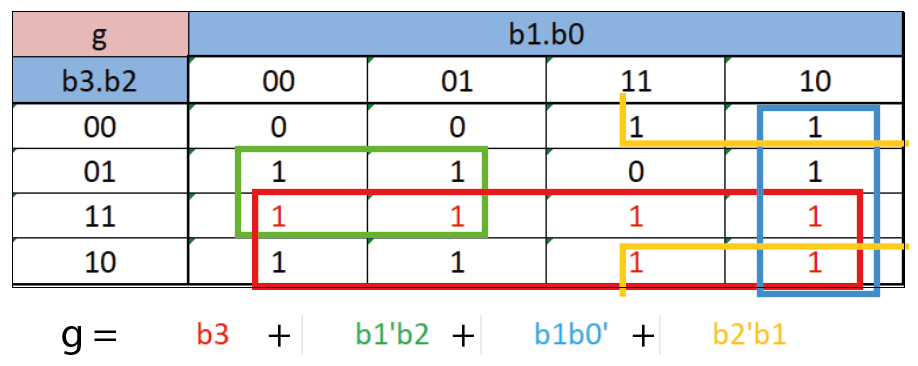
\includegraphics[width=0.9\textwidth]{IMG/tab_de_K_7.png}
    \caption{\textit{Tableau de Karnaugh} - 7}
    \label{fig:colorpicker}
\end{figure}
\medskip

On peut donc poser les solutions sous forme de listes qu'on pourra interpréter respectivement via les index de \texttt{0} à \texttt{6} pour les segments de \texttt{a} à \texttt{g}.
\begin{lstlisting}
s = (b[3] or b[1] or b[0] and b[2] or not b[0] and not 
     b[2],
     b[0] and b[1] or not b[1] and not b[0] or not b[2],
     b[2] or b[3] or not b[1] or b[0],
     b[3] or b[1] and not b[0] or not b[2] and not b[0] 
     or not b[1] and b[0] and b[2] or b[1] and not b[2],
     b[1] and not b[0] or not b[0] and not b[2],
     b[3] or not b[0] and b[2] or not b[1] and b[2] 
     or not b[1] and not b[0],
     b[3] or b[1] and not b[0] or not b[1] and b[2] 
     or not b[2] and b[1])
\end{lstlisting}
\medskip

Puis la liste \texttt{SEG\_MAP} me permet de fixer la position des segments en posant leur coordonnées dans la matrice d'un chiffre digital :
\begin{lstlisting}
SEG_MAP = (((0, 0), (0, 1), (0, 2), (0, 3)), # a
           ((0, 3), (1, 3), (2, 3)), # b
           ((2, 3), (3, 3), (4, 3)), # c
           ((4, 0), (4, 1), (4, 2), (4, 3)), # d
           ((4, 0), (3, 0), (2, 0)), # e
           ((2, 0), (1, 0), (0, 0)), # f
           ((2, 0), (2, 1), (2, 2), (2, 3)), # g
           ((1, 0), (3, 0))) # :
\end{lstlisting}
\medskip

Notez que la dernière ligne correspond au caractère de séparation \og \texttt{:}\fg{} entre l'heure et les minutes.
\medskip

\subsubsection*{\textbullet{} Affichage d'un \textit{digit}}
La variable \texttt{digit} est un tableau \textit{Numpy} initialisé avec des espaces :
\begin{verbatim}
digit = full((5, 6), [" "],dtype=str)
\end{verbatim}
\medskip

Je teste ici avec \texttt{match case} les caractères à afficher, soit \texttt{" "} pour un \textit{digit} \og éteint\fg{}, puis les deux points (\og \texttt{:}\fg{}) pour le séparateur et le reste pour les chiffres de 0 à 9.
\begin{verbatim}
match el:
        case " ": ...
        case ":":
            ...
        case _:
            ...
\end{verbatim}
\medskip

Une fois les solutions de ma table de vérité trouvées, alors on récupère les coordonnées pour afficher un \og \texttt{\#}\fg{} à chaque fois pour former les segments à allumer :
\begin{lstlisting}
digit[*zip(*[(r, c) for i, el in enumerate(s) if el
                 for r, c in SEG_MAP[i]])] = "#"
    return digit
\end{lstlisting}
\medskip

Cette fonction peut être éclatée de cette manière pour plus de lisibilité :
\begin{lstlisting}
pos = [(r, c) for i, el in enumerate(s) if el 
           for r, c in SEG_MAP[i]]
r, c = zip(*pos)
digit[r, c] = "#"
\end{lstlisting}
\medskip

Ce n'est qu'une simple transposition afin de réunir les coordonnées \texttt{x} et \texttt{y} et les appliquer d'un coup et ainsi remplir le tableau \textit{Numpy} \texttt{digit}.
\medskip

\subsubsection*{\textbullet{} Afficher sur une ligne}
Pour ce faire on doit procéder à une lecture ligne par ligne de chaque \texttt{digit}. On utilise pour cela la fonction \texttt{hstack()}\footnote{\url{https://numpy.org/doc/stable/reference/generated/numpy.hstack.html}} qui permet de concaténer ligne par ligne mes tableaux \textit{Numpy}.
\medskip

Tout se fait à cette ligne :
\begin{verbatim}
hstack([display(el) for el in time])
\end{verbatim}
\medskip

\subsubsection*{\textbullet{} Afficher l'heure en suivant l'énoncé}
L'affichage de l'heure n'est pas bien complexe: heure sur un chiffre et les minutes avec deux chiffres. Il faut penser à effacer le premier zéro de l'heure si l'heure est entre 0 et 9 puis d'ajouter un \textit{digit} blanc pour l'affichage.
\begin{lstlisting}
time = datetime.now().strftime("%H:%M").lstrip("0")
...
...time if len(time) == 5 else " "+time...
\end{lstlisting}
\medskip

Pour cela je cherche la taille de l'heure et si l'on a que cinq caractères alors on se trouve dans le cas d'un affichage avec deux \textit{digits} pour l'heure sinon ce sera une longueur de quatre :
\begin{itemize}
	\item[-] 3:24 <- une longueur de quatre
	\item[-] 15h58 <- une longueur de cinq
\end{itemize}
\medskip

Le caractère spécial \og \texttt{:}\fg{} est calculé au sein de la fonction \texttt{display()} en ajoutant une solution supplémentaire pour afficher les positions de mon \og deux-points\fg{} à la fin de la liste \texttt{SEG\_MAP}.
\medskip

\chapter{Cryptographie symétrique}
\vspace{2cm}
\section{Énoncé}
Un peu d'encryptage pour vos communications privées !
\medskip

Le but de ce challenge est de développer un codeur/décodeur suivant la logique de la cryptographie symétrique\footnote{\url{https://fr.wikipedia.org/wiki/Cryptographie_sym\%C3\%A9trique}} qui utilise une clef numérique très simple pour chiffrer et déchiffrer.
\medskip

\subsection*{Étapes}
\begin{enumerate}
	\item Envoyer la phrase à chiffrer : \og \textit{Salut, je suis ici pour apprendre Python}\fg{} et la clef de codage est égale à \texttt{6}.
	\medskip
	
	\item On remplace d'abord tous les espace par des \og \texttt{\_}\fg{}, ce qui nous donne alors la phrase : \og \textit{Salut,\_je\_suis\_ici\_pour\_apprendre\_Python}\fg{}.
	\medskip
	
	\item Comme la clef est la valeur \texttt{6}, on découpe la phrase en lignes de six caractères, les cases manquantes sont comblées par des \og \texttt{*}\fg{}:
	\begin{verbatim}
	Salut,
	_je_su
	is_ici
	_pour_
	appren
	dre_Py
	thon**
	\end{verbatim}
	\medskip

	\item On transpose en lisant le texte par colonne (de haut en bas et de gauche à droite), c'est-à-dire en suivant cet ordre :
	\begin{verbatim}
	1  8 15 22
	2  9 16 23
	3 10 17 24
	4 11 18 25
	5 12 19 26
	6 13 20 27
	7 14 21 28
	\end{verbatim}
\end{enumerate}
\medskip

La phrase chiffrée sera donc la suivante : \og \texttt{S\_i\_adtajspprhle\_opeou\_iur\_ntscreP
*,ui\_ny*}\fg{}.
\medskip

Pour le décodage, il suffira de suivre les étapes dans le sens inverse...
\medskip

\subsection*{Conditions}
\begin{itemize}
	\item[-] L'affichage se fait via la console.
	\item[-] La phrase a chiffrer est a envoyer en argument, accompagnée de sa clef au format \texttt{int}, le résultat doit retourner la phrase codée.
	\item[-] Pour le décodeur, la phrase chiffrée est envoyée accompagnée de la clef, le résultat doit retourner la phrase en clair.
	\item[-] La clef doit être la même pour un même chiffrage et déchiffrage.
	\item[-] Vous êtes libre de coder en fonctionnel ou bien de constituer vos classes à l'aide de la POO.
\end{itemize}
\medskip

\subsection*{Exemples}
\textbf{\textbullet{} Chiffrage}
\begin{itemize}
	\item[-] \og \textit{Lorem ipsum dolor sit amet, consectetur adipiscing elit.}\fg{}, clef : \texttt{12} -> \texttt{Ldetnoot
	ugrl,r\_eo\_\_emrcal\_\_odiisnitpisp.stei*u\_cs*matc*\_mei*}
	\item[-] \og \textit{La première machine programmable a été réalisé en 1801.}\fg{}, clef : \texttt{3} -> \texttt{Lpmrmher
	rmlatrlén8.arieai\_oaae\_ééi\_\_0*\_eè\_cnpgmb\_é\_ase11*}
\end{itemize}
\medskip

\textbf{\textbullet{} Déchiffrage}
\begin{itemize}
	\item[-] \texttt{Lag\_eeelelm*\_l\_aa*ced\_i*hnesn*}, clef : \texttt{5} -> \og \textit{Le challenge de la semaine}\fg{}
	\item[-] \texttt{dctigosrn*}, clef : \texttt{2} -> \og \textit{docstring}\fg{}
\end{itemize}
\medskip

\section{Diverses solutions}
\subsection*{Code de \textbf{\textit{@Arnadu}}}
J'aimerais mettre en avant la meilleure façon d'aborder ce challenge. Et c'est le participant \textbf{\textit{@Arnadu}} qui l'a trouvé ! Après quelques étapes de \textit{refactoring}, voici le code résultant final que je trouve absolument brillant de simplicité et d'ingéniosité.
\medskip

\begin{lstlisting}
def encode(sentence:str, key:int)->str:
    sentence += "*"*(key - len(sentence) % key) \
        if len(sentence) % key else ""
    return "".join(sentence[i::key]
                   for i in range(key)).replace(" ", "_")


def decode(sentence_encrypt:str, key:int)->str:
    cutter = len(sentence_encrypt)//key
    return ("".join(sentence_encrypt[i::cutter]
                   for i in range(cutter))
            .replace("_", " ").rstrip("*"))


sentences_to_encode = (
    ("Lorem ipsum dolor sit amet, consectetur adipiscing "
     "elit.", 12),
    ("La première machine programmable a été réalisé en "
     "1801.", 3)
)

sentences_to_decode = (
    ("Lag_eeelelm*_l_aa*ced_i*hnesn*", 5),
    ("dctigosrn*", 2)
)

for sentence, key in sentences_to_encode:
    print(f"Sentence to encode : {sentence}")
    print(f"Sentence encoded : {encode(sentence, key)}")

for sentence, key in sentences_to_decode:
    print(f"Sentence to decode : {sentence}")
    print(f"Sentence decoded : {decode(sentence, key)}")
\end{lstlisting}
\medskip

Pourquoi son code est excellent ? Car en une seule boucle, il a été capable de réaliser à la fois le découpage et la transposition de la phrase à coder ou à décoder :
\begin{verbatim}
...sentence[i::key] for i in range(key)
\end{verbatim}
\medskip

On récupère donc chaque groupe de caractères à chaque découpage , pour chaque ligne en utilisant la boucle \texttt{for} et \texttt{range(key)} avec l'utilisation d'un pas : \texttt{[i::key]}.
\medskip

Ceci est valable aussi pour le décodage :
\begin{verbatim}
cutter = len(sentence_encrypt)//key
...sentence_encrypt[i::cutter] for i in range(cutter)
\end{verbatim}
\medskip

\subsection*{Le code de \textbf{\textit{@Hugo}}}
Voici une autre solution intéressante avec Numpy en fonctionnel, que je trouve aussi très sympathique. C'est une version sur laquelle nous avons pas mal bossé avec \textbf{\textit{@Hugo}} :
\begin{lstlisting}
import numpy as np


def init_matrix(sentence: str, key: int, decodage=False) \
        -> str:
    x, y = np.ceil(len(sentence)/key).astype(int), key
    if decodage:
        x, y = y, x

    matrix = np.full((x, y), '*')
    for i, c in enumerate(sentence):
        matrix[i//y, i % y] = c
    return ''.join(np.ravel(np.transpose(matrix)))


def code(sentence: str, key: int) -> str:
    return init_matrix(sentence, key).replace(' ','_')


def decode(coded_sentence: str, key: int) -> str:
    return (init_matrix(coded_sentence, key, True)
            .replace('_', ' ').rstrip('*'))


if __name__ == "__main__":
    key = 6
    print(decode(code("Salut, je suis ici pour apprendre "
                      "Python", key), key))
\end{lstlisting}
\medskip

\texttt{x} et \texttt{y} permettent de calculer la dimension de la matrice ; comme le chiffrage et le déchiffrage sont simplement l'inverse, cela peut se faire via une simple permutation des variables pour le décodage.
\medskip

Pour le reste, on initialise une matrice que l'on rempli au fur et à mesure avec la phrase à coder ou à décoder.
\medskip

Une transposition avec \texttt{transpose()} de \textit{Numpy} et \texttt{ravel()} pour aplatir la matrice dans le but d'afficher son contenu.
\medskip

\subsection*{Ma solution}
Voici maintenant ma proposition que je vous laisse analyser et qui est une autre façon de faire avec quelques subtilités intéressantes au niveau du formatage avec \textit{f-string} et de l'utilisation de la fonction \texttt{zip()} :
\begin{lstlisting}
def encode(text: str, key: int)-> str:
    t = [f"{text[i:i + key]:*<{key}}"
         for i in range(0, len(text), key)]
    return "".join("".join(el)
                   for el in zip(*t)).replace(" ", "_")


def decode(text: str, key: int)-> str:
    row = len(text) // key
    t = [text[i:i + row] for i in range(0, len(text), row)]
    return ("".join("".join(el)
                   for el in zip(*t)).rstrip("*").
            replace("_", " "))


key = 6
print(decode(encode("Salut, je suis ici pour apprendre "
                    "Python", key), key))
\end{lstlisting}
\medskip

Ici, la phrase est découpée avec un \textit{pas} de \texttt{key} en utilisant \texttt{range(0, len(text), key)}, puis les caractères sont récupérés ligne par ligne entre l'\textit{index} et l'\textit{index} auquel on ajoute la valeur de \texttt{key}, grâce à \texttt{text[i:i + key]}.
\medskip

On procède ensuite à la transposition à l'aide de la fonction \texttt{zip()} et l'\textit{unpack} (la petite astérisque qui dispatche tous les éléments...) de la compréhension de liste issue de la ligne de code précédente. C'est à ce moment-là que les espaces sont remplacés par des \og \texttt{\_}\fg{}. À noter que pour compléter les espaces vides avec des astérisques, j'utilise ici le formatage à l'aide des \textit{f-string}\footnote{Pour plus d'information sur les \textit{f-string}: \url{https://he-arc.github.io/livre-python/fstrings/index.html}} qui permet de réaliser la fonction via  \texttt{:*<{key}}.
\medskip

Le décodage se fait de la même façon, dans le sens inverse.
\medskip

\subsection*{La solution de \textbf{\textit{@OsKaR31415}}}
\og \textit{Voici ma solution avec le paradigme orienté objet :}
\begin{lstlisting}
import numpy as np
from abc import ABC, abstractmethod


def read_by_columns(str_array: np.ndarray[str]) -> str:
    """Retourner une chaîne de caractère de tous les
    caractères du tableau 2D, lus par colonnes.
    Exemples:
        >>> read_by_columns(np.array([["s", "u"],
        ["a", "t"], ["l", "!"]]))
        'salut!'
    """
    return ''.join(np.ravel(np.transpose(str_array)))

class Codeur(ABC):
    """Classe abstraite pour un objet qui encode ou décode
    un texte avec une clef. Cette classe gère la
    manipulation de la clef (initialisation, accesseur et
    mutateur). Elle pose la nécessité de définir la méthode
    `__call__` dans toutes les classes enfant.
    """
    def __init__(self, clef):
        self.clef = clef

    @property
    def clef(self) -> int:
        return self._clef

    @clef.setter
    def clef(self, valeur: int) -> None:
        if not isinstance(valeur, int):
            raise TypeError(f"La clef doit être un entier"
                            f", pas un {type(valeur)}.")
        self._clef = valeur

    @abstractmethod
    def __call__(self, texte: str) -> str:
        """Une méthode abstraite n'est pas définie.
        Elle sert à dire que toutes les classes filles
        doivent définir cette méthode."""
        ...


class Encodeur(Codeur):
    """Classe pour encoder du texte.
    Puisqu'elle hérite de `Codeur`, il n'est pas nécessaire
    de s'occuper de la gestion de l'attribut `clef`, ni de
    définir le `__init__`."""
    def __call__(self, texte: str) -> str:
        # remplacement des espaces + ajout des "*" à la fin
        texte = (texte.replace(' ', '_') +
                 "*" * (self.clef - len(texte)
                        % self.clef))
        return read_by_columns(np.reshape(np.array(
            list(texte)), (len(texte)//self.clef,
                           self.clef)))

class Decodeur(Codeur):
    """Classe pour décoder du texte."""
    def __call__(self, texte: str) -> str:
        return (read_by_columns(np.reshape(np.array(
            list(texte)), (self.clef, len(texte)//
                           self.clef)))
                .rstrip('*').replace('_', ' '))


chiffrer = Encodeur(12)  # un encodeur avec la clef 12
assert chiffrer("Lorem ipsum dolor sit amet, consectetur "
                "adipiscing elit.") == ("Ldetnootugrl,r_e"
                                        "o__emrcal__odii"
                                        "snitpisp.stei*u_"
                                        "cs*matc*_mei*")
chiffrer.clef = 3  # on change la clef
assert (chiffrer("La première machine programmable a été "
                "réalisé en 1801.") ==
        ("Lpmrmherrmlatrlén8.arieai_oaae_ééi__0*_eè_cnpg"
         "mb_é_ase11*"))

# on peut également définir le Codeur à la volée :
assert (Decodeur(5)("Lag_eeelelm*_l_aa*ced_i*hnesn*") ==
        "Le challenge de la semaine")

# en définissant l'encodeur et le décodeur à la volée :
texte = "un texte au hasard avec un * pour le piège"
clef = 7
assert Decodeur(clef)(Encodeur(clef)(texte)) == texte
\end{lstlisting}
\medskip

\textit{J'ai choisi de faire des objets avec une clef fixée, mais qui peuvent encoder ou décoder n'importe quel texte. Les objets \texttt{Encode} et \texttt{Decode} sont en fait des sortes de fonctions (des \texttt{\_callable\_}) que l'on appelle avec comme argument un texte, et qui vont retourner le texte encodé ou décodé avec leur clef.}\fg{}
\medskip

\section[Quelques remarques sur les codes des participants]{Quelques remarques sur les codes des \newline participants au challenge, par \newline \textbf{\textit{@OsKaR31415}}}
Quelques remarques sur les codes que j'ai vu :
\medskip

Parmi les solutions, certaines utilisaient parfois trois boucles, et beaucoup de calculs intermédiaires. C'est une bonne pratique de diviser un problème en petits sous-problèmes (\og \textit{diviser chacune des difficultés [...] en autant de parcelles qu'il se pourrait, et qu'il serait requis pour les mieux résoudre}\fg{} comme disait \textsc{Descartes}).
\medskip

Mais il ne faut pas en abuser : trop diviser son code pose problème. D'abord, cela ajoute de la complexité puisqu'il faut réunir les différentes parties divisées. Mais surtout, c'est problématique car on est souvent obligés, pour pouvoir le diviser, de rendre le problème plus complexe qu'il ne l'est.
\medskip

C'est une question de cacher le code (par exemple le mettre dans une fonction à part), ou bien de le subordonner (ne pas le séparer, mais faire en sorte que sa délimitation soit claire, avec des parenthèses ou des variables). Par exemple, \textbf{@bucdany} à tendance à faire des lignes plutôt longues car il est à l'aise avec le code subordonné : une compréhension de liste dans une fonction, suivie d'un \texttt{.replace}... Si on est habitué, c'est plus lisible qu'un code dans lequel chaque étape est séparée dans une fonction à part.
\medskip

J'ai vu plusieurs solutions utilisant la programmation orientée objet. C'est un paradigme très utile et pratique, mais il faut aussi comprendre sa logique. Par exemple, dans ce challenge, il fallait gérer un texte et une clef pour l'encodage et le décodage. Certaines solutions ont été de faire un objet qui contient un texte, et de proposer de (dé/en)coder ce texte avec n'importe quelle clef. Cela peut être utile dans certains contexte, mais généralement, il semble plus logique de choisir une clef une fois, et ensuite d'encoder plusieurs textes. Pour cela, mes classes ne stockent pas le texte, mais le transforment simplement.
\medskip

Il faut penser à ce genre d'enjeux lorsque l'on définit la structure de nos objets. Il faut aussi repérer les parties du code qui seront communes à plusieurs classes pour en faire une classe parente.
\medskip

Enfin, les classes abstraites peuvent être utiles lorsque l'on veut définir un \\
\texttt{\_contrat\_}, c'est à dire une sorte de structure que toutes les classes filles d'une classe doivent respecter. Dans mon code, la classe \texttt{Codeur} est une classe abstraite (elle ne sert pas à créer des objets, mais d'autres classes peuvent hériter d'elle), et elle pose le contrat suivant : toutes les classes filles doivent contenir la méthode \texttt{\_\_call\_\_}.
\medskip

\section{Partie \textit{bonus} du challenge}
Le mot clé n'est plus de type \texttt{int} mais de type \texttt{string} de \texttt{n} caractères. On prendra ici le mot clé de six caractères : \texttt{python}.
\medskip

\subsection*{Étapes}
\begin{enumerate}
	\item On fera alors bien correspondre chaque lettre de ce dernier, à notre phrase à coder que l'on découpera en \texttt{n} caractères (la longueur de notre mot clé) de cette manière :
	\begin{verbatim}
p y t h o n
S a l u t ,
_ j e _ s u
i s _ i c i
_ p o u r _
a p p r e n
d r e _ P y
t h o n * *
	\end{verbatim}
	\medskip
	
	\item On range ensuite chaque lettre du mot clé par ordre alphabétique : \texttt{h n o p t y}. Chaque lettre de la phrase à coder sera alors mélangée de sorte qu'elle suive toujours sa correspondance avec la lettre du mot clé qui lui a été associée dans la phase précédente. On aura donc ce résultat :
	\begin{verbatim}
h n o p t y
u , t S l a
_ u s _ e j
i i c i _ s
u _ r _ o p
r n e a p p
_ y P d e r
n * * t o h
	\end{verbatim}
	\medskip
	
	\item Pour finir, on lira le tout par colonne (en veillant bien sûr à enlever du traitement, la première ligne, c'est-à-dire, notre mot clé) pour obtenir la phrase codée suivante :
	\begin{verbatim}	 u_iur_n,ui_ny*tscreP*S_i_adtle_opeoajspprh
	\end{verbatim}
\end{enumerate}
\medskip

Bien sûr, je vous invite à créer une méthode de décodage en repassant toutes les étapes dans l'ordre inverse...
\medskip

Là, ça devient un algorithme de cryptage plutôt intéressant et vraiment pas facile à décoder sans la clé !
\medskip

\textbf{NOTA}: Afin d'éviter d'avoir des problèmes au décodage, je vous invite à faire vos tests en veillant à ne pas choisir un mot clé qui possède des récurrences dans sa constitution : par exemple, pour le mot clé : \texttt{"probleme"}, les deux \texttt{"e"} contenus dans ce mot peuvent être rangés dans un ordre alphabétique différent, laissant alors deux résultats possibles...
\medskip

Bonne chance !

\end{document}